\chapter{Introduction\label{cha:intro}}
\epigraph{Learning is not a product of schooling, but the lifelong attempt to
acquire it.}{\textit{Albert Einstein}}
\noindent
%1215

Simply defined by the European Commission \citeyearpar{EuropeanCommission2000},
\LLLs represents all learning activities throughout lives of individuals aimed
at improving their knowledge and skills. The concept of \LLLs has become very
popular over the last decade. The original concept has gone through a lot of
changes, through the stages of continuing, recurrent, and adult education
\citep{Jarvis2004}. On one hand, the \LLLs concept has an entirely economic
agenda, where citizens can be described as tools for economic development and
their needs are firmly tied to the needs of industry
\citep[pp.~112-114]{Carter2008}. On the other hand, as stated by UNESCO, \LLLs
is a cultural policy which influences the nature of society and promotes
positive change \citep[pp.~12-14]{Boshier2000}. However, no matter which point
of view is adopted, world economics, employment patterns and societies are
changing with the increasing importance of \LLLs
\citep{Jarvis2008,Simmons-McDonald2009}. For full participation in education,
workplace, and society, people today require well-developed \LLLs skills,
developed from the early stages of their lives \citep{Otala1997}.

In addition to being a subject for political and economic discussion
\citep{Bagnall2009}, \LLLs has been established as a topic of interest in
higher education, in particular universities \citep{Knapper2000}. In attempt to
provide support for \LLLsn, many universities are currently trying out various
approaches. Among these are changing institutional policies, developing graduate
profiles, and establishing cross-sector collaboration models.

\citet{Duke2001} claims application of information technology to learning to be
the major factor that put \LLLs on the agenda of higher education. From the
perspective of the technical solutions available today, the IT revolution
brought the new means of accessing and delivering information for both teaching
and learning purposes. Numerous systems and frameworks emerged aimed at
supporting various learning activities. 

As a result, the field of technology created for learning is currently
over-saturated with such terms as learning management systems, course management
systems, virtual learning environments, \ep~systems, personal learning
environments, Web 2.0 technologies, and other terms. In relation to the context
of this thesis, all of them provide some kind of support for learning, whether
it is by facilitating assessment, as a tool for exchanging information, or in
any other way. However, is supporting learning the same as supporting
\textit{lifelong} learning? Can the same tools be used to support both? Or is
there a need for more comprehensive solutions?

In light of the importance of \LLLs and focusing on the role of universities,
this research project will try to answer these questions by exploring ways
of addressing the need for \LLLs support in universities.

\section{Research Goal}

The overall aim of this research is to design and implement a learner-centred
e-learning environment which will support and facilitate the \LLLs process in
universities. This research project suggests improving an \ep~system as a part
of the institutional learning environment, where learning management system
(LMS) currently dominates. \ep s are learner focused and have the potential of
supporting all types of learning, including the ones outside of scope of formal
education. A review of this field will establish that the \ep~systems are
already used in universities, sometimes in connection with LMS. This research
explores whether these systems adequately meet the requirements of both
students, lecturers and education providers (universities) as \LLLs
stakeholders.

\section{Research Design}

This research follows a well established methodology in the field of ICT Design
Science Research (DSR). This methodology is fundamentally a problem-solving
approach \citep{Cross1993} which is well suited with the goal of this research.
Going through the stages of identifying the problem, suggesting solutions,
design and development, evaluation and conclusion
\citep{Peffers2008,Vaishnavi2007}, this research project explores the various
aspects of \LLLs support in universities and creates a background for bringing a
sound technology to students which addresses their needs in the first place.

This research is primarily qualitative due to the lack of previous research (as
will be demonstrated in the course of this thesis) and the \LLLs context of this
project which by its nature is not suited to quantitative measures
\citep{Creswell2009}. However, it also employs quantitative methods for the 
evaluation stage to improve the chances of getting a wide range of feedback and
achieve a better understanding of the potential issues.

\section{Scope and Limitations}

Although technology is usually called a key driver of educational change
\citep{Attwell2007}, one can argue that in the context of \LLLs this phenomenon
is not only a technical question \citep{Schaffert2008}. Many other changes
should occur to fully implement \LLLs in universities: changes in the way of
thinking of both students and lecturers, support on the higher (department or
institutional) levels, provision of technical support and professional
development for staff, personal motivation of learners, etc. As technology is
one of the components of fully supported \LLLs environment, this project is
focused on technical aspects. The other aspects are outside of the scope of
this research. However, state of the art literature and theories in the area
are still comprehensively investigated.

\section{Thesis Structure and Outline}

The remainder of this thesis is structured as follows (Figure \ref{fig:ts}):

\begin{figure}[htb]
\centering
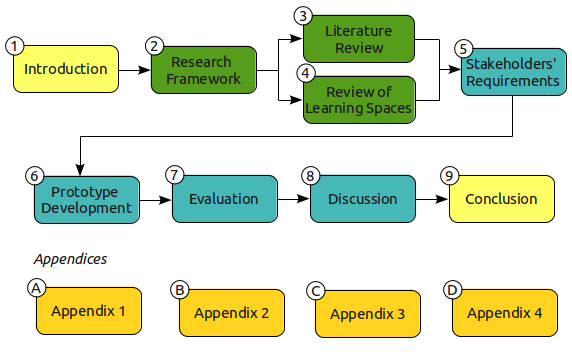
\includegraphics[width=0.9\textwidth]{CH1-F1-Thesis}
\caption{Thesis structure}
\label{fig:ts}
\end{figure}

\begin{description}
\item[Chapter 2.] This chapter presents a methodological approach employed in
this research. Theoretical background of design science research methodology is
given and the way this approach was adopted in this project is described.
\item[Chapter 3.] This chapter focuses on discussing the background of
\LLLsn. Its connection to universities, the current situation in this area and
the problems associated with \LLLs in universities are shown here.
\item[Chapter 4.] This chapter explores the technical worlds of learning
support. System that are currently employed at universities are examined according
to their compliance with \LLLs support.
\item[Chapter 5.] The results of literature review (Chapter 3) and a review of
learning spaces (Chapter 4) are taken to the stakeholders for analysis of their
needs and requirements. Later these findings are used in development of a
conceptual model of an environment that can provide support for \LLLsn.
\item[Chapter 6.] A prototype implementation (based on the requirements
developed in Chapter 5) process and outcomes are presented in this chapter.
\item[Chapter 7.] This chapter describes a complex evaluation design used in the
research to address the questions of quality, functionality and suitability of
the developed features.
\item[Chapter 8.] In this chapter the results and lessons learnt are discussed
with an attempt to analyse issues and question the outcomes. Technical
considerations and practical applications of this research are presented.
\item[Chapter 9.] This chapter brings conclusions and contributions of the
research presented in this thesis. It explores implications for theory and
practice as well as the potential for future research.
\end{description}

This thesis also includes a number of appendices, namely:

\begin{description}
\item[Appendix A] provides ethics documentation for the first stage of the
requirements analysis.
\item[Appendix B] gives an overview of the documents used in the stakeholders
interviews, such as questions used in the interviews and scenarios discussed
with the participants.
\item[Appendix C] consists of the formal requirements specification used for
development of the prototype features. This specification is developed in the
form of user stories.
\item[Appendix D] includes interface screenshots of the prototype features. 
\item[Appendix E] provides ethics documentation for the evaluation stage of this
research project.
\item[Appendix F] overviews the documents used in evaluation Study Two (group
experiment) which includes study protocol, background and exit questionnaire,
participants' responses and the examples of their work.
\item[Appendix G] overviews the documents used in evaluation Study Three (case
studies) which includes study protocol, background questionnaire, and interview
questions.
\end{description}